% Official contribution: https://conferences.iaea.org/event/498/contributions/43620/
% Scheduled date: 2026-10-27.
\paragraph{Abstract}
This presentation reviews the modernisation of IAEA Nuclear Data Dissemination Services, focusing on the Nuclear Reaction Data Explorer \url{https://nds.iaea.org/dataexplorer} and its supporting workflows~\cite{dataexplorer}. The backend converts EXFOR records into JSON~\url{https://github.com/IAEA-NDS/exfor_json} and SQL database, and tabulated data files~\cite{EXFORTABLES-py} for retrieval and visualisation (Figure~\ref{fig:so-dataflow}). Developments include broader observable coverage, visualization of various observables, library comparisons, access to historical evaluations powered by DeCE code~\cite{Kawano2019DeCE} (Figure~\ref{fig:so-dece}), bibliographic and reaction-index searches for EXFOR entries, (Figure~\ref{fig:so-stat}) and APIs.
\begin{figure}[htbp]
    \centering  
    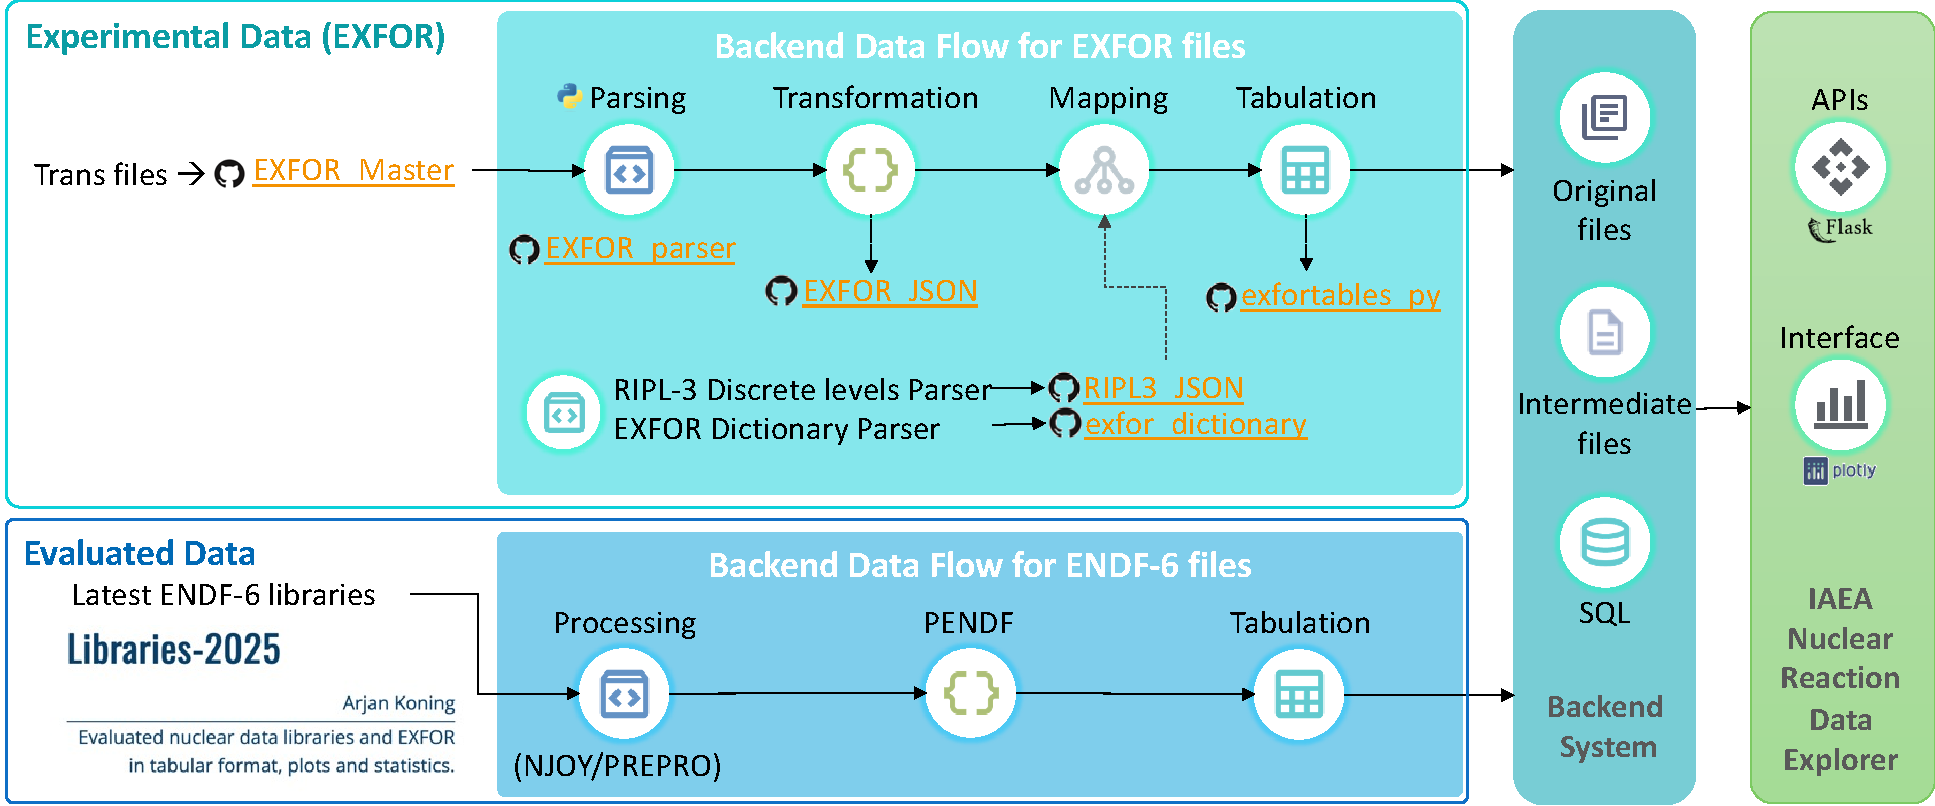
\includegraphics[width=0.6\textwidth]{figures/okumura-dataflow.pdf}
    \caption{Dataflow: Experimental (EXFOR) and Evaluated (ENDF-6) Data}
    \label{fig:so-dataflow}
\end{figure}
\begin{figure}[htbp]
    \centering  
    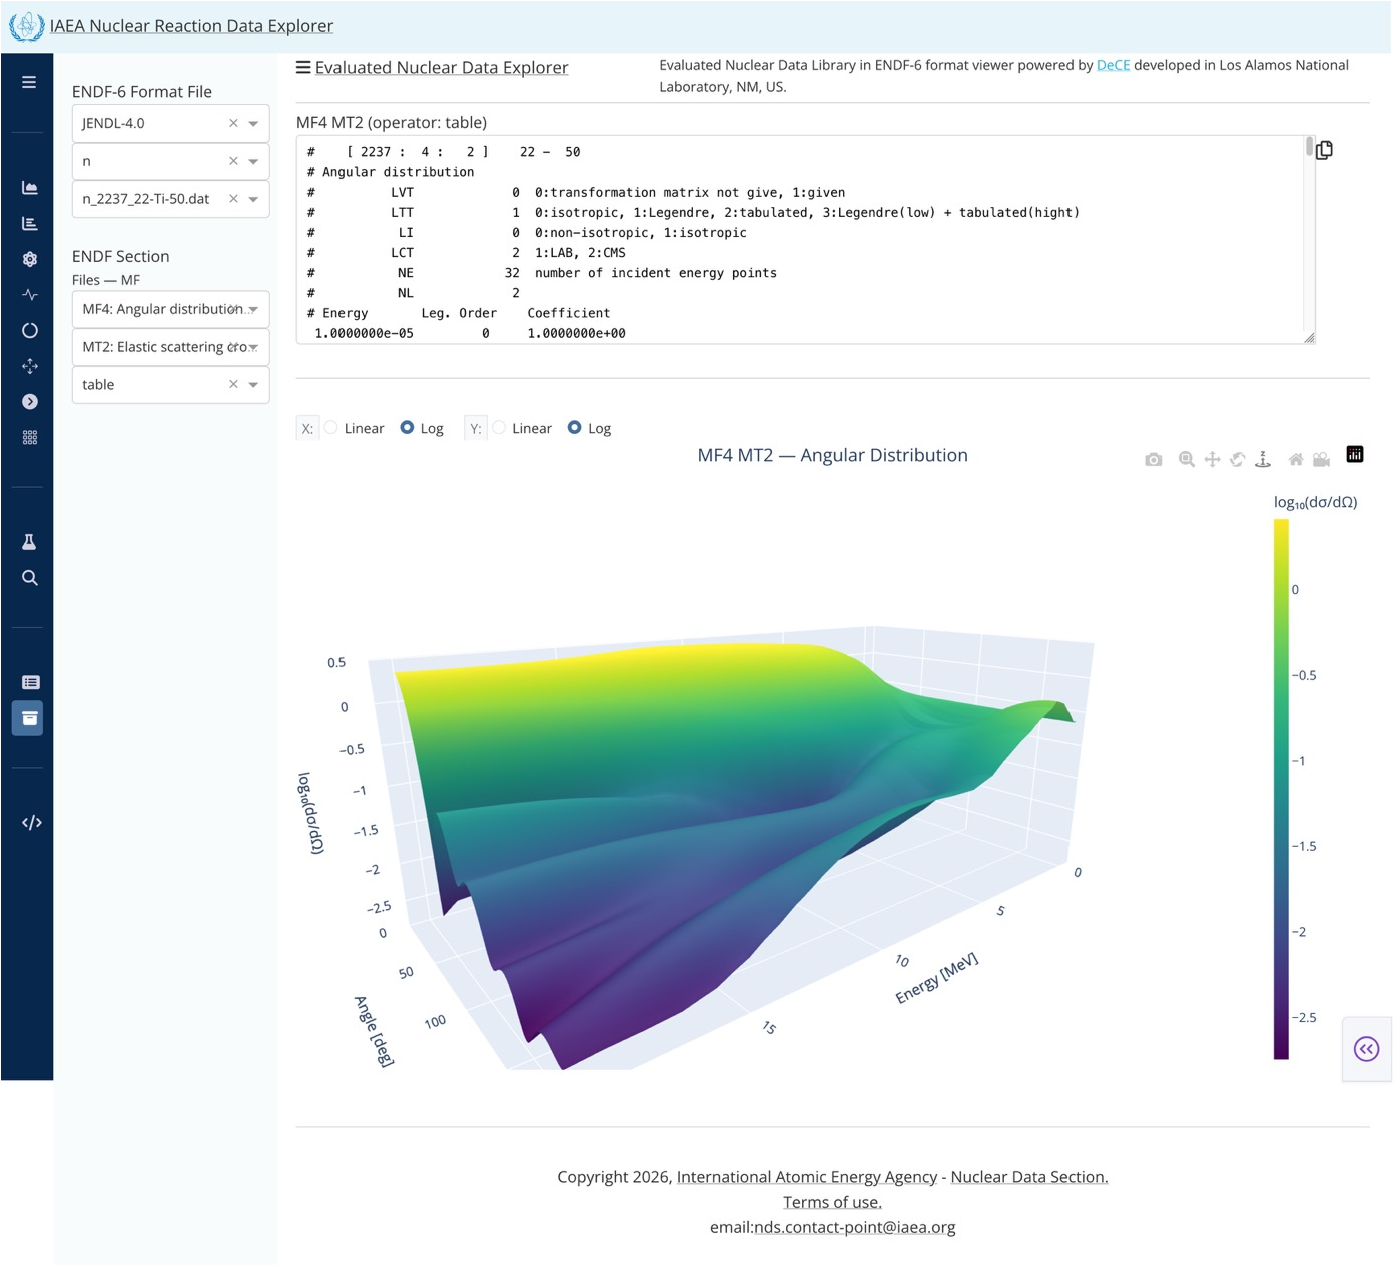
\includegraphics[width=0.6\textwidth]{figures/okumura-dece.pdf}
    \caption{Access to historical evaluations powered by DeCE code~\cite{Kawano2019DeCE}}
    \label{fig:so-dece}
\end{figure}
\begin{figure}[htbp]
    \centering  
    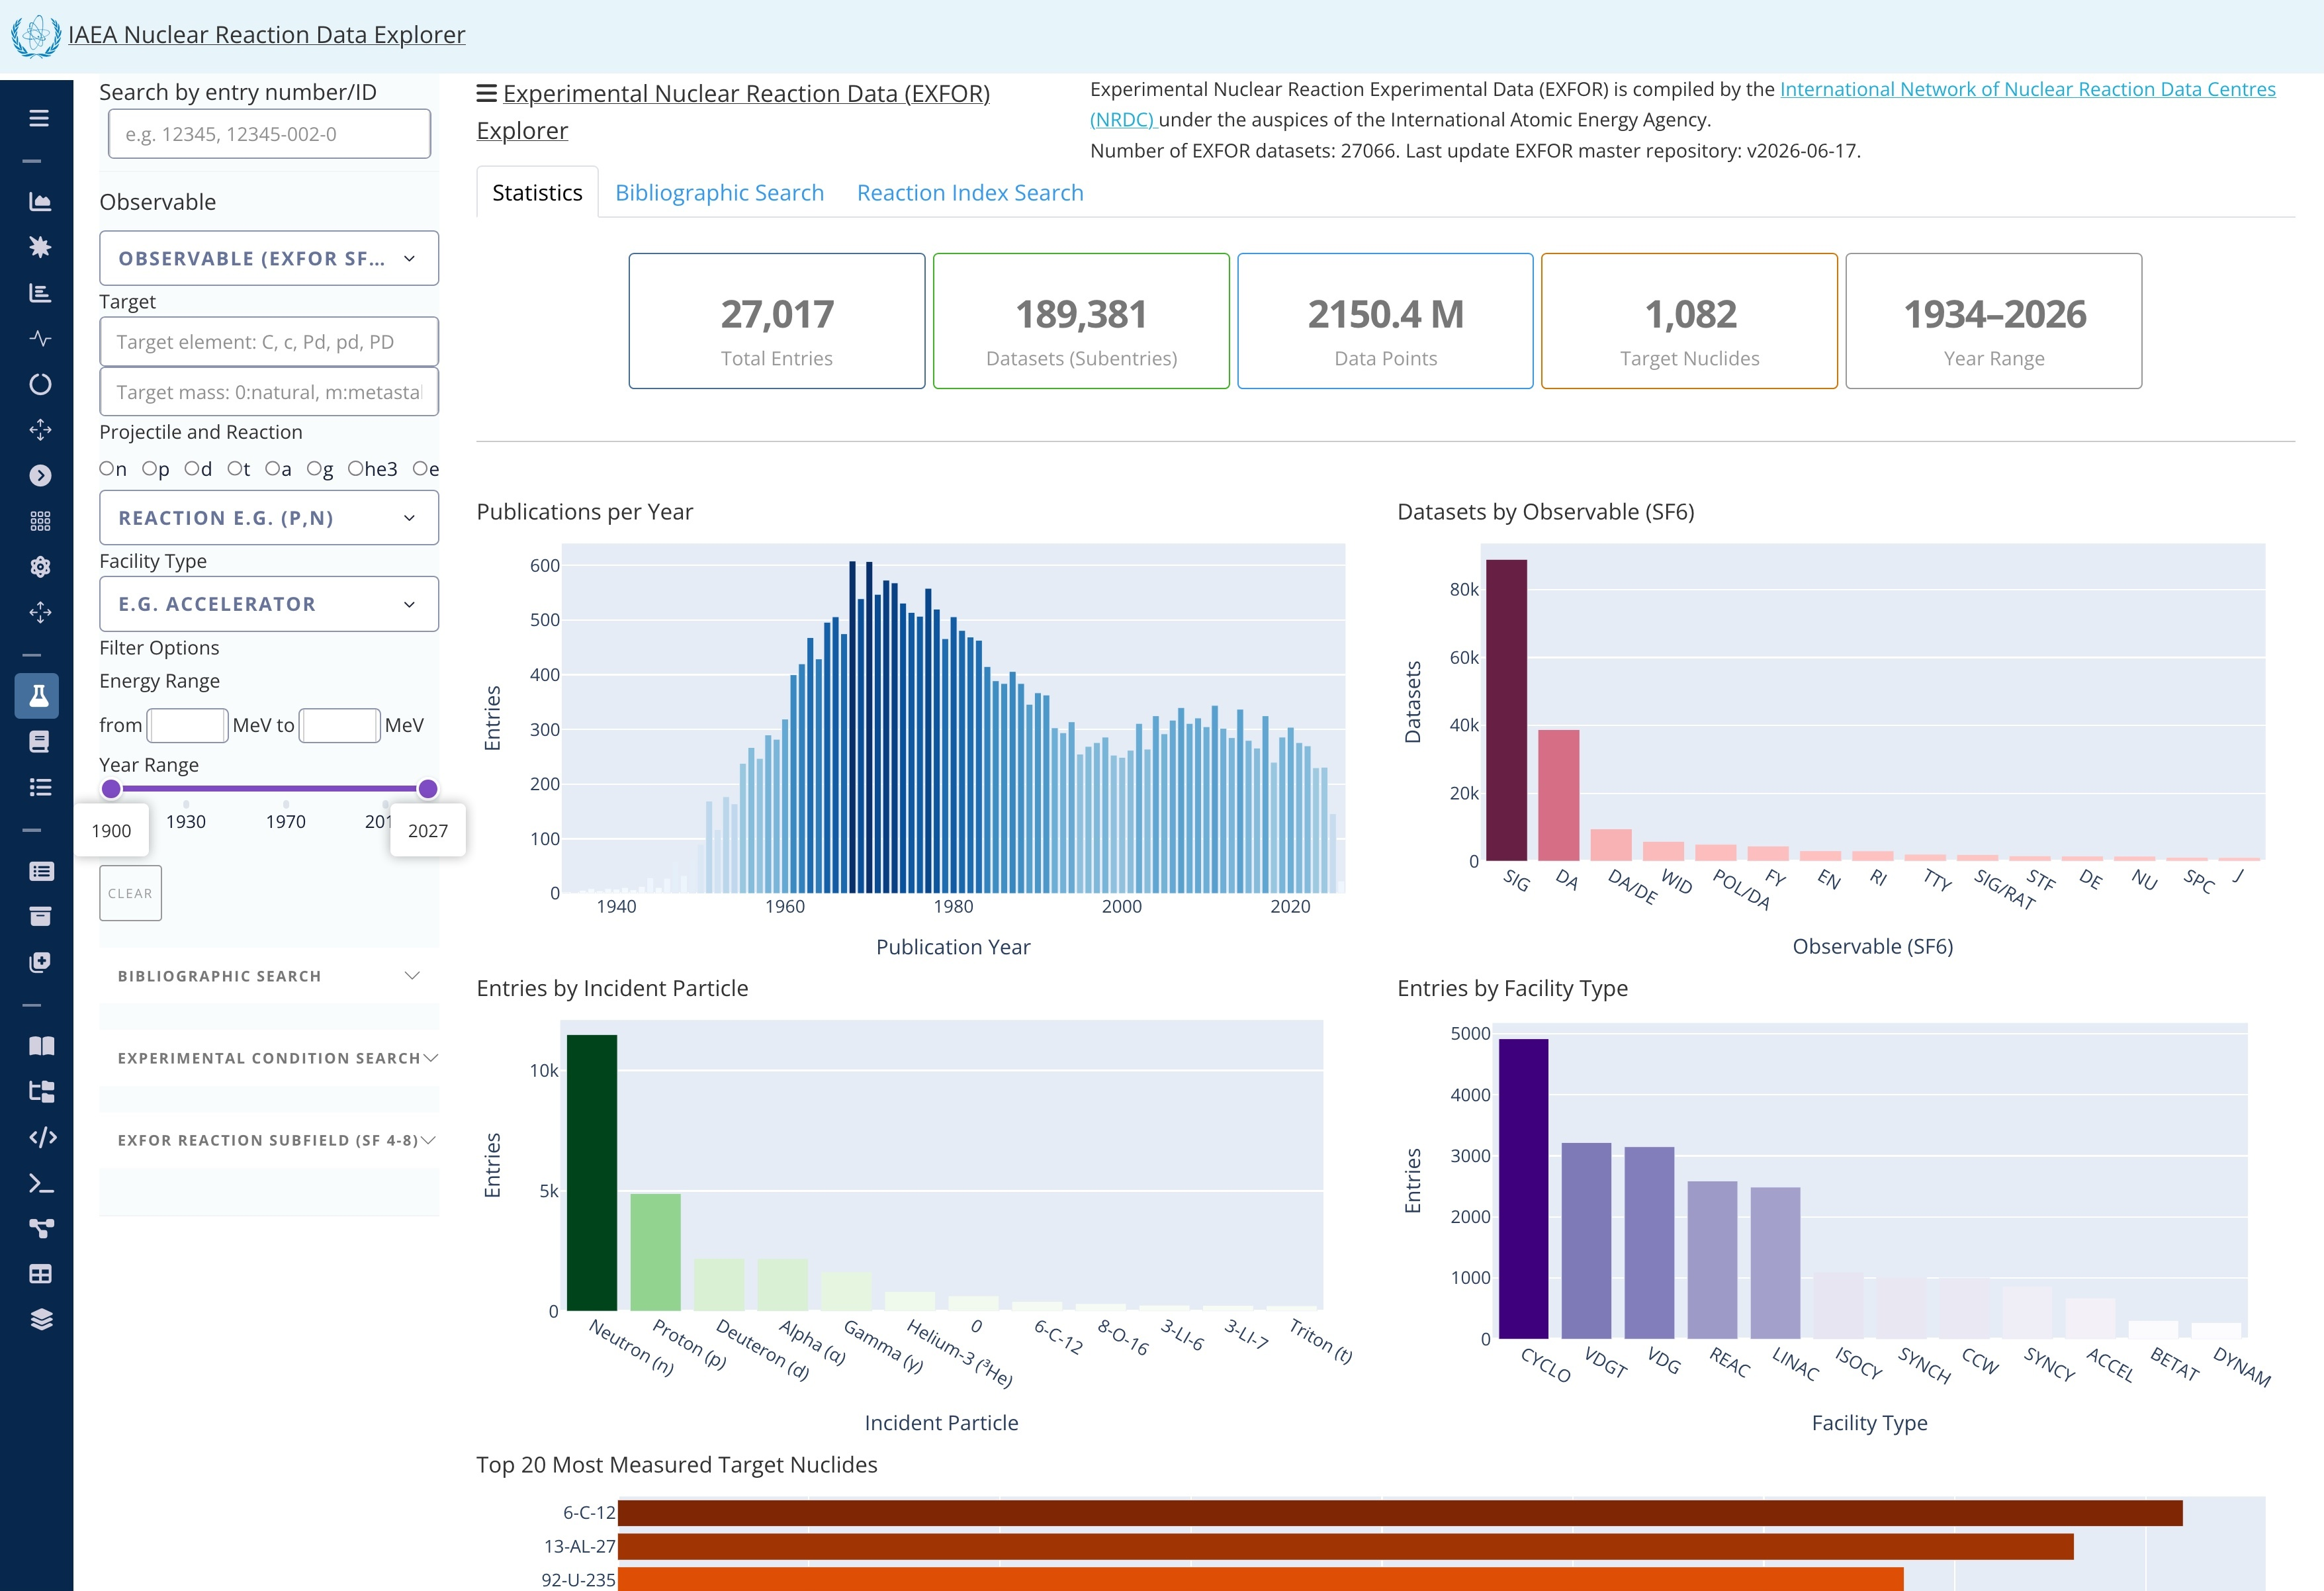
\includegraphics[width=0.75\textwidth]{figures/okumura-exfor-statistics.jpg}
    \caption{EXFOR Statistics}
    \label{fig:so-stat}
\end{figure}


A complementary workflow recovers missing publication DOIs from EXFOR bibliographic information~\cite{exfor-entry-doi}. It uses title and author matching through Crossref, together with lookup rules for coded journal and report references. The scope includes main references, related references and monitor references. Existing identifiers are preserved, and the source of entry-level additions is recorded. Similarity-based matches remain heuristic and require stronger bibliographic checks and review of ambiguous candidates.

The presentation also introduces a community-contribution prototype on Data Portal Project linking submitted or revised datasets to publications and EXFOR records, and tests of migrating legacy NDS resources to Invenio~\cite{invenio}. These developments address data discovery, provenance, reuse and long-term maintenance. Further work includes production deployment, automated updates, completeness checks, moderation workflows and verification that migration preserves data and associated resources.
\mbox{}\par

\paragraph{Discussion}
Shin Okumura demonstrated Data Explorer's access to experimental and evaluated data through parsed records, tabulated observables, plots and APIs. Discussion covered filtering, library comparisons, plot controls and links back to source records. 

Participants also suggested comparison with users' local data, including browser-side handling and temporary uploads. Storage, authentication and review arrangements for a broader submission service remained open until the IAEA officially provides new SSO service such as NUCLEUS. 